% Options for packages loaded elsewhere
\PassOptionsToPackage{unicode}{hyperref}
\PassOptionsToPackage{hyphens}{url}
%
\documentclass[
]{article}
\title{RegresionLogistica\_FugaClientes}
\author{Laura Piñeros}
\date{Febrero\_2022}

\usepackage{amsmath,amssymb}
\usepackage{lmodern}
\usepackage{iftex}
\ifPDFTeX
  \usepackage[T1]{fontenc}
  \usepackage[utf8]{inputenc}
  \usepackage{textcomp} % provide euro and other symbols
\else % if luatex or xetex
  \usepackage{unicode-math}
  \defaultfontfeatures{Scale=MatchLowercase}
  \defaultfontfeatures[\rmfamily]{Ligatures=TeX,Scale=1}
\fi
% Use upquote if available, for straight quotes in verbatim environments
\IfFileExists{upquote.sty}{\usepackage{upquote}}{}
\IfFileExists{microtype.sty}{% use microtype if available
  \usepackage[]{microtype}
  \UseMicrotypeSet[protrusion]{basicmath} % disable protrusion for tt fonts
}{}
\makeatletter
\@ifundefined{KOMAClassName}{% if non-KOMA class
  \IfFileExists{parskip.sty}{%
    \usepackage{parskip}
  }{% else
    \setlength{\parindent}{0pt}
    \setlength{\parskip}{6pt plus 2pt minus 1pt}}
}{% if KOMA class
  \KOMAoptions{parskip=half}}
\makeatother
\usepackage{xcolor}
\IfFileExists{xurl.sty}{\usepackage{xurl}}{} % add URL line breaks if available
\IfFileExists{bookmark.sty}{\usepackage{bookmark}}{\usepackage{hyperref}}
\hypersetup{
  pdftitle={RegresionLogistica\_FugaClientes},
  pdfauthor={Laura Piñeros},
  hidelinks,
  pdfcreator={LaTeX via pandoc}}
\urlstyle{same} % disable monospaced font for URLs
\usepackage[margin=1in]{geometry}
\usepackage{color}
\usepackage{fancyvrb}
\newcommand{\VerbBar}{|}
\newcommand{\VERB}{\Verb[commandchars=\\\{\}]}
\DefineVerbatimEnvironment{Highlighting}{Verbatim}{commandchars=\\\{\}}
% Add ',fontsize=\small' for more characters per line
\usepackage{framed}
\definecolor{shadecolor}{RGB}{248,248,248}
\newenvironment{Shaded}{\begin{snugshade}}{\end{snugshade}}
\newcommand{\AlertTok}[1]{\textcolor[rgb]{0.94,0.16,0.16}{#1}}
\newcommand{\AnnotationTok}[1]{\textcolor[rgb]{0.56,0.35,0.01}{\textbf{\textit{#1}}}}
\newcommand{\AttributeTok}[1]{\textcolor[rgb]{0.77,0.63,0.00}{#1}}
\newcommand{\BaseNTok}[1]{\textcolor[rgb]{0.00,0.00,0.81}{#1}}
\newcommand{\BuiltInTok}[1]{#1}
\newcommand{\CharTok}[1]{\textcolor[rgb]{0.31,0.60,0.02}{#1}}
\newcommand{\CommentTok}[1]{\textcolor[rgb]{0.56,0.35,0.01}{\textit{#1}}}
\newcommand{\CommentVarTok}[1]{\textcolor[rgb]{0.56,0.35,0.01}{\textbf{\textit{#1}}}}
\newcommand{\ConstantTok}[1]{\textcolor[rgb]{0.00,0.00,0.00}{#1}}
\newcommand{\ControlFlowTok}[1]{\textcolor[rgb]{0.13,0.29,0.53}{\textbf{#1}}}
\newcommand{\DataTypeTok}[1]{\textcolor[rgb]{0.13,0.29,0.53}{#1}}
\newcommand{\DecValTok}[1]{\textcolor[rgb]{0.00,0.00,0.81}{#1}}
\newcommand{\DocumentationTok}[1]{\textcolor[rgb]{0.56,0.35,0.01}{\textbf{\textit{#1}}}}
\newcommand{\ErrorTok}[1]{\textcolor[rgb]{0.64,0.00,0.00}{\textbf{#1}}}
\newcommand{\ExtensionTok}[1]{#1}
\newcommand{\FloatTok}[1]{\textcolor[rgb]{0.00,0.00,0.81}{#1}}
\newcommand{\FunctionTok}[1]{\textcolor[rgb]{0.00,0.00,0.00}{#1}}
\newcommand{\ImportTok}[1]{#1}
\newcommand{\InformationTok}[1]{\textcolor[rgb]{0.56,0.35,0.01}{\textbf{\textit{#1}}}}
\newcommand{\KeywordTok}[1]{\textcolor[rgb]{0.13,0.29,0.53}{\textbf{#1}}}
\newcommand{\NormalTok}[1]{#1}
\newcommand{\OperatorTok}[1]{\textcolor[rgb]{0.81,0.36,0.00}{\textbf{#1}}}
\newcommand{\OtherTok}[1]{\textcolor[rgb]{0.56,0.35,0.01}{#1}}
\newcommand{\PreprocessorTok}[1]{\textcolor[rgb]{0.56,0.35,0.01}{\textit{#1}}}
\newcommand{\RegionMarkerTok}[1]{#1}
\newcommand{\SpecialCharTok}[1]{\textcolor[rgb]{0.00,0.00,0.00}{#1}}
\newcommand{\SpecialStringTok}[1]{\textcolor[rgb]{0.31,0.60,0.02}{#1}}
\newcommand{\StringTok}[1]{\textcolor[rgb]{0.31,0.60,0.02}{#1}}
\newcommand{\VariableTok}[1]{\textcolor[rgb]{0.00,0.00,0.00}{#1}}
\newcommand{\VerbatimStringTok}[1]{\textcolor[rgb]{0.31,0.60,0.02}{#1}}
\newcommand{\WarningTok}[1]{\textcolor[rgb]{0.56,0.35,0.01}{\textbf{\textit{#1}}}}
\usepackage{graphicx}
\makeatletter
\def\maxwidth{\ifdim\Gin@nat@width>\linewidth\linewidth\else\Gin@nat@width\fi}
\def\maxheight{\ifdim\Gin@nat@height>\textheight\textheight\else\Gin@nat@height\fi}
\makeatother
% Scale images if necessary, so that they will not overflow the page
% margins by default, and it is still possible to overwrite the defaults
% using explicit options in \includegraphics[width, height, ...]{}
\setkeys{Gin}{width=\maxwidth,height=\maxheight,keepaspectratio}
% Set default figure placement to htbp
\makeatletter
\def\fps@figure{htbp}
\makeatother
\setlength{\emergencystretch}{3em} % prevent overfull lines
\providecommand{\tightlist}{%
  \setlength{\itemsep}{0pt}\setlength{\parskip}{0pt}}
\setcounter{secnumdepth}{-\maxdimen} % remove section numbering
\ifLuaTeX
  \usepackage{selnolig}  % disable illegal ligatures
\fi

\begin{document}
\maketitle

\hypertarget{aplicaciuxf3n-del-modelo}{%
\subsection{Aplicación del modelo}\label{aplicaciuxf3n-del-modelo}}

En primer lugar se fija el directorio de trabajo donde tenemos las
funciones y los datos.

Procedemos a la lectura de los datos depurados.

\begin{Shaded}
\begin{Highlighting}[]
\CommentTok{\# Parto de los datos sin atípicos ni ausentes guardados}
\NormalTok{datos}\OtherTok{\textless{}{-}}\FunctionTok{readRDS}\NormalTok{(}\StringTok{"C:/Users/Laura/Desktop/UCM/Documentacion2/Tarea/datosFugaClientes.RDS"}\NormalTok{)}
\CommentTok{\#names(datos)}
\NormalTok{varObjBin}\OtherTok{\textless{}{-}}\NormalTok{datos}\SpecialCharTok{$}\NormalTok{varObjBin}
\NormalTok{input}\OtherTok{\textless{}{-}}\NormalTok{datos[,}\SpecialCharTok{{-}}\NormalTok{(}\DecValTok{1}\NormalTok{)]}
\end{Highlighting}
\end{Shaded}

Variables control:

\begin{Shaded}
\begin{Highlighting}[]
\CommentTok{\# Creo la variable aleatoria}
\NormalTok{input}\SpecialCharTok{$}\NormalTok{aleatorio}\OtherTok{\textless{}{-}}\FunctionTok{runif}\NormalTok{(}\FunctionTok{nrow}\NormalTok{(input))}
\NormalTok{input}\SpecialCharTok{$}\NormalTok{aleatorio2}\OtherTok{\textless{}{-}}\FunctionTok{runif}\NormalTok{(}\FunctionTok{nrow}\NormalTok{(input))}
\FunctionTok{str}\NormalTok{(input)}
\end{Highlighting}
\end{Shaded}

\begin{verbatim}
## 'data.frame':    6353 obs. of  23 variables:
##  $ ID             : num  4858 3587 2338 4997 5879 ...
##  $ Genero         : Factor w/ 2 levels "Female","Male": 1 2 2 1 1 1 2 1 2 2 ...
##  $ Mayor65        : Factor w/ 2 levels "0","1": 1 1 1 1 1 1 1 1 1 1 ...
##  $ Conyuge        : Factor w/ 2 levels "No","Yes": 2 1 1 1 1 1 1 1 2 1 ...
##  $ PersCargo      : Factor w/ 2 levels "No","Yes": 1 1 1 1 1 1 2 1 1 2 ...
##  $ Antiguedad     : num  1 34 2 45 22.1 ...
##  $ Telf_serv      : Factor w/ 2 levels "No","Yes": 1 2 2 1 2 2 2 1 2 2 ...
##  $ VariasLineas   : Factor w/ 2 levels "No","Yes": 1 1 1 1 1 2 2 1 2 1 ...
##  $ Int_serv       : Factor w/ 3 levels "DSL","Fiber optic",..: 1 1 1 1 2 2 2 2 2 1 ...
##  $ Seguridad      : Factor w/ 2 levels "No","Yes": 1 2 2 2 1 1 1 2 1 2 ...
##  $ CopiaSeguridad : Factor w/ 2 levels "No","Yes": 2 1 2 1 1 1 2 1 1 2 ...
##  $ Antivirus_disp : Factor w/ 2 levels "No","Yes": 1 2 1 2 1 2 1 1 2 1 ...
##  $ Soporte_tecnico: Factor w/ 2 levels "No","Yes": 1 1 1 2 1 1 1 1 2 1 ...
##  $ TV_streaming   : Factor w/ 2 levels "No","Yes": 1 1 1 1 1 2 2 1 2 1 ...
##  $ Peliculas      : Factor w/ 2 levels "No","Yes": 1 1 1 1 1 2 1 1 2 1 ...
##  $ Contrato       : Factor w/ 3 levels "Month-to-month",..: 1 2 1 2 1 1 1 1 1 2 ...
##  $ Fact_sinPapel  : Factor w/ 2 levels "No","Yes": 2 1 2 1 2 2 2 1 2 1 ...
##  $ MetodoPago     : Factor w/ 4 levels "Bank transfer (automatic)",..: 1 4 4 1 3 2 2 4 3 1 ...
##  $ FacturaMes     : num  76.6 20.6 53.9 42.3 70.7 ...
##  $ FacturaTotal   : num  29.9 1889.5 108.2 1840.8 151.7 ...
##  $ prop_missings  : num  0.1 0.05 0 0.1 0.05 0.05 0.05 0.05 0.05 0.1 ...
##  $ aleatorio      : num  0.7199 0.7856 0.1454 0.9902 0.0991 ...
##  $ aleatorio2     : num  0.6462 0.3835 0.1055 0.0687 0.0519 ...
\end{verbatim}

\hypertarget{estudio-descriptivo-de-relaciones-con-la-respuesta}{%
\subsection{Estudio descriptivo de relaciones con la
respuesta}\label{estudio-descriptivo-de-relaciones-con-la-respuesta}}

En este apartado intentaremos descubrir a priori las relaciones
marginales de las variables con la variable objetivo binaria para
hacernos una idea de cuales de ellas serán potencialmente influyentes en
los modelos de regresión logística que ajustemos.

\begin{Shaded}
\begin{Highlighting}[]
\CommentTok{\#Obtengo la importancia de las variables. }
\CommentTok{\#Falla si hay alguna variable cuantitativa con menos de 6 valores diferentes}
\NormalTok{input}\SpecialCharTok{$}\NormalTok{prop\_missings }\OtherTok{\textless{}{-}}\FunctionTok{as.factor}\NormalTok{(input}\SpecialCharTok{$}\NormalTok{prop\_missings)}
\FunctionTok{graficoVcramer}\NormalTok{(input,varObjBin)}
\end{Highlighting}
\end{Shaded}

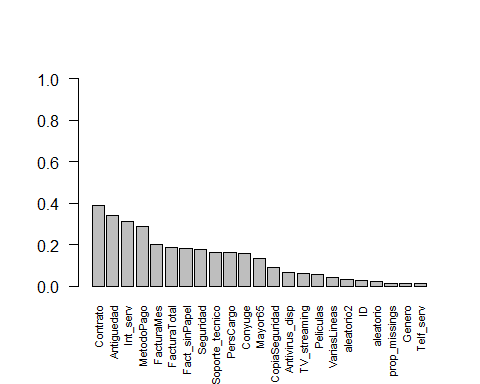
\includegraphics{RegresionLog_FugaClientes_files/figure-latex/Vcramer-1.pdf}

Podemos decir que las variables tentativas para el modelado son:

\begin{itemize}
\tightlist
\item
  Contrato
\item
  Antiguedad
\item
  Int\_serv
\item
  MetodoPago
\end{itemize}

Después de aleatorio2 empezamos a sospechar que las relaciones con la
variable objetivo si pueden ser casualidad.

Veamos gráficamente la relacion entre las varaibles con la objetivo, por
medio del mosaico. Tomemos una variable que ifluye y tomemos otra que no
tanto a ver que nos resulta.

\begin{Shaded}
\begin{Highlighting}[]
\CommentTok{\#Veo gráficamente el efecto de dos variables cualitativas sobre la binaria}
\NormalTok{m1}\OtherTok{\textless{}{-}}\FunctionTok{mosaico\_targetbinaria}\NormalTok{(input}\SpecialCharTok{$}\NormalTok{Peliculas,varObjBin,}\StringTok{"Peliculas"}\NormalTok{) }\CommentTok{\#esta no influye }
\end{Highlighting}
\end{Shaded}

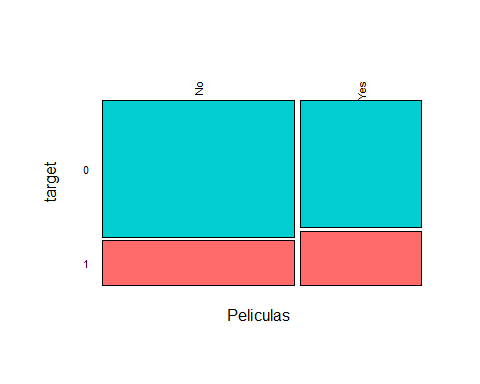
\includegraphics{RegresionLog_FugaClientes_files/figure-latex/mosaicos-1.pdf}

\begin{Shaded}
\begin{Highlighting}[]
\NormalTok{m2}\OtherTok{\textless{}{-}}\FunctionTok{mosaico\_targetbinaria}\NormalTok{(input}\SpecialCharTok{$}\NormalTok{Contrato,varObjBin,}\StringTok{"Contrato"}\NormalTok{) }\CommentTok{\#esta sí influye}
\end{Highlighting}
\end{Shaded}

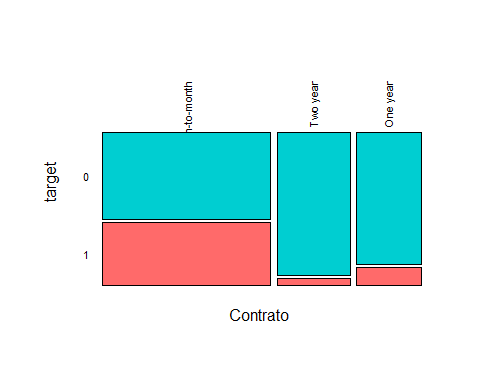
\includegraphics{RegresionLog_FugaClientes_files/figure-latex/mosaicos-2.pdf}

Para la variable peliculas, que no tiene mucha incidencia podemos ver
que hay una mínima diferencia entre las regiones. Para la variable
Contrato, que consideramos tiene mucha incidencia con la variable
objetivo, es más probable contrato con objetivo uno, cuando es mes a
mes. Parece ser que, el contrato extendido por un año y hasta dos años,
puede darnos indicio de fuga de clientes.

Veamos que efecto tienen dos variables cuantitativas sobre la objetivo
binaria.

\begin{Shaded}
\begin{Highlighting}[]
\CommentTok{\#Veo gráficamente el efecto de dos variables cuantitativas sobre la binaria}
\NormalTok{bx1}\OtherTok{\textless{}{-}}\FunctionTok{boxplot\_targetbinaria}\NormalTok{(input}\SpecialCharTok{$}\NormalTok{Antiguedad,varObjBin,}\StringTok{"Antiguedad"}\NormalTok{)}
\NormalTok{bx2}\OtherTok{\textless{}{-}}\FunctionTok{boxplot\_targetbinaria}\NormalTok{(input}\SpecialCharTok{$}\NormalTok{FacturaMes,varObjBin,}\StringTok{"FacturaMes"}\NormalTok{)}
\NormalTok{bx4}\OtherTok{\textless{}{-}}\FunctionTok{boxplot\_targetbinaria}\NormalTok{(input}\SpecialCharTok{$}\NormalTok{FacturaTotal,varObjBin,}\StringTok{"FacturaTotal"}\NormalTok{)}


\NormalTok{h1}\OtherTok{\textless{}{-}}\FunctionTok{hist\_targetbinaria}\NormalTok{(input}\SpecialCharTok{$}\NormalTok{Antiguedad,varObjBin,}\StringTok{"Antiguedad"}\NormalTok{)}
\NormalTok{h2}\OtherTok{\textless{}{-}}\FunctionTok{hist\_targetbinaria}\NormalTok{(input}\SpecialCharTok{$}\NormalTok{FacturaMes,varObjBin,}\StringTok{"FacturaMes"}\NormalTok{)}
\NormalTok{h4}\OtherTok{\textless{}{-}}\FunctionTok{hist\_targetbinaria}\NormalTok{(input}\SpecialCharTok{$}\NormalTok{FacturaTotal,varObjBin,}\StringTok{"FacturaTotal"}\NormalTok{)}

\FunctionTok{marrangeGrob}\NormalTok{(}\FunctionTok{list}\NormalTok{(bx1,bx2,h1,h2),}\AttributeTok{nrow =} \DecValTok{2}\NormalTok{,}\AttributeTok{ncol =} \DecValTok{2}\NormalTok{)}
\end{Highlighting}
\end{Shaded}

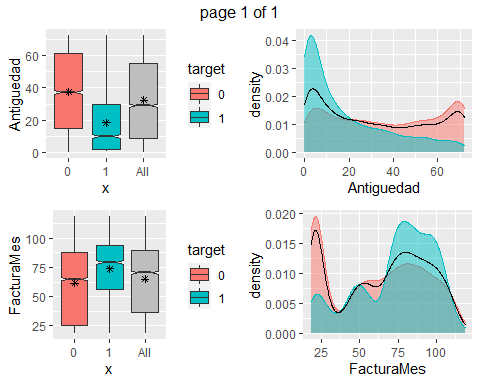
\includegraphics{RegresionLog_FugaClientes_files/figure-latex/histogramas y boxplots-1.pdf}

\begin{Shaded}
\begin{Highlighting}[]
\FunctionTok{marrangeGrob}\NormalTok{(}\FunctionTok{list}\NormalTok{(bx4,h4),}\AttributeTok{nrow =} \DecValTok{1}\NormalTok{,}\AttributeTok{ncol =} \DecValTok{2}\NormalTok{)}
\end{Highlighting}
\end{Shaded}

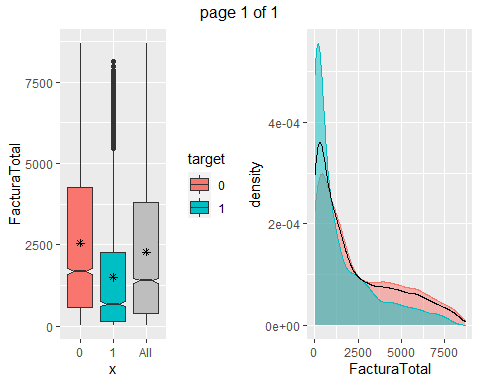
\includegraphics{RegresionLog_FugaClientes_files/figure-latex/histogramas y boxplots-2.pdf}
Los graficos Vcramer nos intenta decir que, para clientes cuyo tiempo de
antiguedad es apenas de unos meses, tienen mas probabilidad de Fuga.
Aquellos clientes que se fugan(fuga=1) no presentan facturas tan altas.
Deben tener un posible sesgo.

\hypertarget{tranformaciones-de-variables}{%
\subsection{Tranformaciones de
variables}\label{tranformaciones-de-variables}}

Vamos a generar las transformaciones de las variable continuas que
maximizan la relación con la variable objetivo binaria en sentido de V
de Cramer.

\begin{Shaded}
\begin{Highlighting}[]
\CommentTok{\#Busco las mejores transformaciones para las variables numéricas con respesto a la variable binaria}
\NormalTok{input\_bin}\OtherTok{\textless{}{-}}\FunctionTok{cbind}\NormalTok{(input,}\FunctionTok{Transf\_Auto}\NormalTok{(}\FunctionTok{Filter}\NormalTok{(is.numeric, input),varObjBin))}

\CommentTok{\# Guardamos el dataset con las tranformaciones}
\NormalTok{todo\_bin}\OtherTok{\textless{}{-}}\FunctionTok{data.frame}\NormalTok{(input\_bin,varObjBin)}
\FunctionTok{saveRDS}\NormalTok{(todo\_bin,}\StringTok{"todo\_bin\_Fuga\_Clientes.RDS"}\NormalTok{)}
\end{Highlighting}
\end{Shaded}

\begin{Shaded}
\begin{Highlighting}[]
\CommentTok{\#Obtengo la importancia de las variables. }
\FunctionTok{graficoVcramer}\NormalTok{(input\_bin,varObjBin)}
\end{Highlighting}
\end{Shaded}

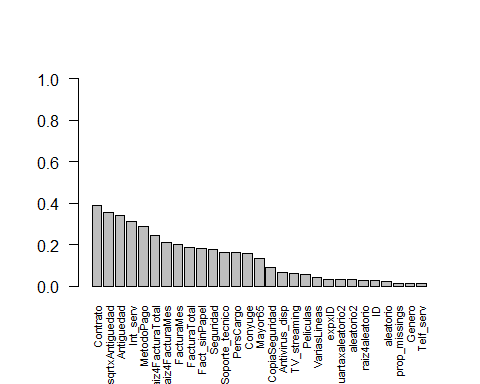
\includegraphics{RegresionLog_FugaClientes_files/figure-latex/Vcramer tranformaciones-1.pdf}
Tiene buena pinta, pues no hubo muchos cambios. Hasta acá, quisimos dar
una breve descripción a los datos para encontar incidencias con la
variable objetivo.

\#\#Modelo de regresión logistica para la predicción de la variable Fuga

\begin{Shaded}
\begin{Highlighting}[]
\CommentTok{\#todo\textless{}{-}readRDS("todo\_bin")}
\NormalTok{todo}\OtherTok{\textless{}{-}}\NormalTok{todo\_bin}

\FunctionTok{freq}\NormalTok{(todo}\SpecialCharTok{$}\NormalTok{varObjBin) }\CommentTok{\#ese ha de ser el error de referencia}
\end{Highlighting}
\end{Shaded}

\begin{verbatim}
##      n    % val%
## 0 4667 73.5 73.5
## 1 1686 26.5 26.5
\end{verbatim}

Siguiendo las especificaciones del modelo, este tendrá mas dificultad en
reconocer a los 1, es decir, los clientes en fuga.

\hypertarget{particiuxf3n-training-test}{%
\subsubsection{Partición
training-test}\label{particiuxf3n-training-test}}

\begin{Shaded}
\begin{Highlighting}[]
\CommentTok{\#Hago la partición}
\FunctionTok{set.seed}\NormalTok{(}\DecValTok{123456}\NormalTok{)}
\NormalTok{trainIndex }\OtherTok{\textless{}{-}} \FunctionTok{createDataPartition}\NormalTok{(todo}\SpecialCharTok{$}\NormalTok{varObjBin, }\AttributeTok{p=}\FloatTok{0.8}\NormalTok{, }\AttributeTok{list=}\ConstantTok{FALSE}\NormalTok{)}
\NormalTok{data\_train }\OtherTok{\textless{}{-}}\NormalTok{ todo[trainIndex,}\FunctionTok{c}\NormalTok{(}\DecValTok{1}\SpecialCharTok{:}\DecValTok{23}\NormalTok{,}\DecValTok{30}\NormalTok{)]}
\NormalTok{data\_test }\OtherTok{\textless{}{-}}\NormalTok{ todo[}\SpecialCharTok{{-}}\NormalTok{trainIndex,}\FunctionTok{c}\NormalTok{(}\DecValTok{1}\SpecialCharTok{:}\DecValTok{23}\NormalTok{,}\DecValTok{30}\NormalTok{)]}
\CommentTok{\#data\_test \textless{}{-} readRDS("C:/Users/Laura/Desktop/UCM/Documentacion2/Tarea/FugaClientes\_test.RDS")}
\end{Highlighting}
\end{Shaded}

Quitemos los efectos no deseados o doblajes de las variables.

\begin{Shaded}
\begin{Highlighting}[]
\CommentTok{\# Este fue el modelo manual ganador }
\NormalTok{modeloManual}\OtherTok{\textless{}{-}}\FunctionTok{glm}\NormalTok{(varObjBin}\SpecialCharTok{\textasciitilde{}}\NormalTok{Contrato}\SpecialCharTok{+}\NormalTok{Int\_serv}\SpecialCharTok{+}\NormalTok{Antiguedad,}
             \AttributeTok{data=}\NormalTok{data\_train,}\AttributeTok{family=}\NormalTok{binomial)}
\FunctionTok{summary}\NormalTok{(modeloManual)}
\end{Highlighting}
\end{Shaded}

\begin{verbatim}
## 
## Call:
## glm(formula = varObjBin ~ Contrato + Int_serv + Antiguedad, family = binomial, 
##     data = data_train)
## 
## Deviance Residuals: 
##     Min       1Q   Median       3Q      Max  
## -1.5710  -0.7222  -0.3248   0.8296   3.0450  
## 
## Coefficients:
##                      Estimate Std. Error z value Pr(>|z|)    
## (Intercept)         -0.258148   0.074173  -3.480 0.000501 ***
## ContratoOne year    -0.885448   0.114614  -7.725 1.11e-14 ***
## ContratoTwo year    -1.562561   0.163289  -9.569  < 2e-16 ***
## Int_servFiber optic  1.180832   0.084704  13.941  < 2e-16 ***
## Int_servNo          -0.868976   0.129198  -6.726 1.75e-11 ***
## Antiguedad          -0.032822   0.002117 -15.506  < 2e-16 ***
## ---
## Signif. codes:  0 '***' 0.001 '**' 0.01 '*' 0.05 '.' 0.1 ' ' 1
## 
## (Dispersion parameter for binomial family taken to be 1)
## 
##     Null deviance: 5882.3  on 5082  degrees of freedom
## Residual deviance: 4435.1  on 5077  degrees of freedom
## AIC: 4447.1
## 
## Number of Fisher Scoring iterations: 6
\end{verbatim}

\begin{Shaded}
\begin{Highlighting}[]
\FunctionTok{pseudoR2}\NormalTok{(modeloManual,data\_train,}\StringTok{"varObjBin"}\NormalTok{)}
\end{Highlighting}
\end{Shaded}

\begin{verbatim}
## [1] 0.2460286
\end{verbatim}

\begin{Shaded}
\begin{Highlighting}[]
\FunctionTok{pseudoR2}\NormalTok{(modeloManual,data\_test,}\StringTok{"varObjBin"}\NormalTok{)}
\end{Highlighting}
\end{Shaded}

\begin{verbatim}
## [1] 0.2259682
\end{verbatim}

\hypertarget{esquema-de-selecciuxf3n-de-variables-por-lasso}{%
\section{Esquema de selección de variables por
Lasso}\label{esquema-de-selecciuxf3n-de-variables-por-lasso}}

\begin{Shaded}
\begin{Highlighting}[]
\DocumentationTok{\#\# LASSO, lo hacemos sin interacciones pues, de lo contrario, puede coger interacciones y no las variables que las forman}
\NormalTok{y }\OtherTok{\textless{}{-}} \FunctionTok{as.double}\NormalTok{(}\FunctionTok{as.matrix}\NormalTok{(data\_train[, }\DecValTok{24}\NormalTok{]))}
\NormalTok{x}\OtherTok{\textless{}{-}}\FunctionTok{model.matrix}\NormalTok{(varObjBin}\SpecialCharTok{\textasciitilde{}}\NormalTok{., }\AttributeTok{data=}\NormalTok{data\_train)[,}\SpecialCharTok{{-}}\DecValTok{1}\NormalTok{]}\CommentTok{\#no cambiar el {-}1}
\FunctionTok{set.seed}\NormalTok{(}\DecValTok{1712}\NormalTok{)}
\NormalTok{cv.lasso }\OtherTok{\textless{}{-}} \FunctionTok{cv.glmnet}\NormalTok{(x,y,}\AttributeTok{nfolds=}\DecValTok{5}\NormalTok{)}
\FunctionTok{plot}\NormalTok{(cv.lasso)}
\end{Highlighting}
\end{Shaded}

\includegraphics{RegresionLog_FugaClientes_files/figure-latex/Lasso-1.pdf}

Este es el comportamiento de lambda y el intervalo de 1se. Mostramos lo
coeficiente.

\begin{Shaded}
\begin{Highlighting}[]
\NormalTok{(betas}\OtherTok{\textless{}{-}}\FunctionTok{coef}\NormalTok{(cv.lasso, }\AttributeTok{s=}\NormalTok{cv.lasso}\SpecialCharTok{$}\NormalTok{lambda}\FloatTok{.1}\NormalTok{se))}
\end{Highlighting}
\end{Shaded}

\begin{verbatim}
## 30 x 1 sparse Matrix of class "dgCMatrix"
##                                              s1
## (Intercept)                        3.496470e-01
## ID                                 .           
## GeneroMale                         .           
## Mayor651                           3.907690e-02
## ConyugeYes                         .           
## PersCargoYes                      -1.934867e-02
## Antiguedad                        -2.489575e-03
## Telf_servYes                      -2.828362e-03
## VariasLineasYes                    3.316130e-02
## Int_servFiber optic                1.568947e-01
## Int_servNo                        -1.111252e-01
## SeguridadYes                      -4.756257e-02
## CopiaSeguridadYes                 -1.149368e-03
## Antivirus_dispYes                  .           
## Soporte_tecnicoYes                -3.723444e-02
## TV_streamingYes                    3.982925e-02
## PeliculasYes                       1.861739e-02
## ContratoOne year                  -9.515854e-02
## ContratoTwo year                  -7.778815e-02
## Fact_sinPapelYes                   4.003716e-02
## MetodoPagoCredit card (automatic)  .           
## MetodoPagoElectronic check         6.329805e-02
## MetodoPagoMailed check             .           
## FacturaMes                         1.475427e-04
## FacturaTotal                      -3.228229e-05
## prop_missings0.05                  .           
## prop_missings0.1                   .           
## prop_missings0.15                  .           
## aleatorio                          .           
## aleatorio2                         .
\end{verbatim}

Note que:

\begin{itemize}
\tightlist
\item
  Hay una buena cantidad de variables que influyen en nuestro modelos,
  las de punto tienen una distripución sobre los parámetros que no vale
  la pena. Habia considerado que la fatura mensual influiría y al
  parecer no. Con seguridad, las variables
\end{itemize}

\begin{Shaded}
\begin{Highlighting}[]
\CommentTok{\#pruebo un primer modelo sin las transformadas}
\NormalTok{modeloInicial}\OtherTok{\textless{}{-}}\FunctionTok{glm}\NormalTok{(varObjBin}\SpecialCharTok{\textasciitilde{}}\NormalTok{.,}\AttributeTok{data=}\NormalTok{data\_train[,}\SpecialCharTok{{-}}\FunctionTok{c}\NormalTok{(}\DecValTok{1}\NormalTok{)],}\AttributeTok{family=}\NormalTok{binomial)}
\FunctionTok{summary}\NormalTok{(modeloInicial)}
\end{Highlighting}
\end{Shaded}

\begin{verbatim}
## 
## Call:
## glm(formula = varObjBin ~ ., family = binomial, data = data_train[, 
##     -c(1)])
## 
## Deviance Residuals: 
##     Min       1Q   Median       3Q      Max  
## -2.0896  -0.6627  -0.3083   0.6799   3.1215  
## 
## Coefficients:
##                                     Estimate Std. Error z value Pr(>|z|)    
## (Intercept)                       -2.469e-01  2.311e-01  -1.068 0.285454    
## GeneroMale                        -3.770e-02  7.657e-02  -0.492 0.622496    
## Mayor651                           2.634e-01  1.016e-01   2.592 0.009532 ** 
## ConyugeYes                        -4.827e-02  9.211e-02  -0.524 0.600269    
## PersCargoYes                      -1.914e-01  1.049e-01  -1.825 0.067977 .  
## Antiguedad                        -2.562e-02  4.056e-03  -6.317 2.67e-10 ***
## Telf_servYes                      -6.442e-01  1.620e-01  -3.976 7.00e-05 ***
## VariasLineasYes                    3.543e-01  9.481e-02   3.738 0.000186 ***
## Int_servFiber optic                8.198e-01  1.288e-01   6.363 1.98e-10 ***
## Int_servNo                        -6.020e-01  1.647e-01  -3.655 0.000257 ***
## SeguridadYes                      -5.028e-01  1.026e-01  -4.902 9.48e-07 ***
## CopiaSeguridadYes                 -2.023e-01  9.406e-02  -2.151 0.031472 *  
## Antivirus_dispYes                 -6.965e-02  9.617e-02  -0.724 0.468935    
## Soporte_tecnicoYes                -3.631e-01  1.029e-01  -3.530 0.000416 ***
## TV_streamingYes                    3.444e-01  1.025e-01   3.359 0.000782 ***
## PeliculasYes                       1.665e-01  1.008e-01   1.651 0.098704 .  
## ContratoOne year                  -7.224e-01  1.200e-01  -6.020 1.75e-09 ***
## ContratoTwo year                  -1.338e+00  1.707e-01  -7.837 4.61e-15 ***
## Fact_sinPapelYes                   3.267e-01  8.607e-02   3.795 0.000147 ***
## MetodoPagoCredit card (automatic) -1.905e-01  1.312e-01  -1.452 0.146536    
## MetodoPagoElectronic check         1.996e-01  1.089e-01   1.833 0.066860 .  
## MetodoPagoMailed check            -2.627e-02  1.274e-01  -0.206 0.836625    
## FacturaMes                         5.880e-03  3.384e-03   1.738 0.082245 .  
## FacturaTotal                      -1.084e-04  5.176e-05  -2.094 0.036247 *  
## prop_missings0.05                  9.121e-02  8.414e-02   1.084 0.278406    
## prop_missings0.1                   4.715e-02  1.566e-01   0.301 0.763434    
## prop_missings0.15                  5.271e-01  4.277e-01   1.233 0.217761    
## aleatorio                         -1.653e-01  1.335e-01  -1.238 0.215663    
## aleatorio2                         1.385e-01  1.331e-01   1.041 0.298057    
## ---
## Signif. codes:  0 '***' 0.001 '**' 0.01 '*' 0.05 '.' 0.1 ' ' 1
## 
## (Dispersion parameter for binomial family taken to be 1)
## 
##     Null deviance: 5882.3  on 5082  degrees of freedom
## Residual deviance: 4234.1  on 5054  degrees of freedom
## AIC: 4292.1
## 
## Number of Fisher Scoring iterations: 6
\end{verbatim}

Consultamos los valores de pseudoR2 en los conjuntos de training y test,

\begin{Shaded}
\begin{Highlighting}[]
\FunctionTok{pseudoR2}\NormalTok{(modeloInicial,data\_train,}\StringTok{"varObjBin"}\NormalTok{)}
\end{Highlighting}
\end{Shaded}

\begin{verbatim}
## [1] 0.2801928
\end{verbatim}

\begin{Shaded}
\begin{Highlighting}[]
\FunctionTok{pseudoR2}\NormalTok{(modeloInicial,data\_test,}\StringTok{"varObjBin"}\NormalTok{)}
\end{Highlighting}
\end{Shaded}

\begin{verbatim}
## [1] 0.2464755
\end{verbatim}

\begin{Shaded}
\begin{Highlighting}[]
\NormalTok{modeloInicial}\SpecialCharTok{$}\NormalTok{rank }\CommentTok{\#número de parámetros}
\end{Highlighting}
\end{Shaded}

\begin{verbatim}
## [1] 29
\end{verbatim}

\begin{Shaded}
\begin{Highlighting}[]
\FunctionTok{impVariablesLog}\NormalTok{(modeloInicial,}\StringTok{"varObjBin"}\NormalTok{) }
\end{Highlighting}
\end{Shaded}

\includegraphics{RegresionLog_FugaClientes_files/figure-latex/unnamed-chunk-5-1.pdf}

\begin{Shaded}
\begin{Highlighting}[]
\CommentTok{\#si los datos de entrenamiento, no se llaman "data\_train", hay que indicarlo}
\end{Highlighting}
\end{Shaded}

En el gráfico se ordenan las aportaciones al pseudoR2 de las distintas
variables teniendo Contrato como la gran ganadora ya que aporta
muchísimo más que cualquiera.

Ahora, considremos un modelo con las 3 primeras variables, pues
presentan incidencias sobre la variable objetivo.

\begin{Shaded}
\begin{Highlighting}[]
\CommentTok{\#pruebo uno sencillo con 3 variables}
\CommentTok{\#glm() modelos lineales generalizados }
\NormalTok{modelo2}\OtherTok{\textless{}{-}}\FunctionTok{glm}\NormalTok{(varObjBin}\SpecialCharTok{\textasciitilde{}}\NormalTok{Contrato}\SpecialCharTok{+}\NormalTok{Int\_serv}\SpecialCharTok{+}\NormalTok{Antiguedad,}
             \AttributeTok{data=}\NormalTok{data\_train,}\AttributeTok{family=}\NormalTok{binomial)}
\FunctionTok{summary}\NormalTok{(modelo2)}
\end{Highlighting}
\end{Shaded}

\begin{verbatim}
## 
## Call:
## glm(formula = varObjBin ~ Contrato + Int_serv + Antiguedad, family = binomial, 
##     data = data_train)
## 
## Deviance Residuals: 
##     Min       1Q   Median       3Q      Max  
## -1.5710  -0.7222  -0.3248   0.8296   3.0450  
## 
## Coefficients:
##                      Estimate Std. Error z value Pr(>|z|)    
## (Intercept)         -0.258148   0.074173  -3.480 0.000501 ***
## ContratoOne year    -0.885448   0.114614  -7.725 1.11e-14 ***
## ContratoTwo year    -1.562561   0.163289  -9.569  < 2e-16 ***
## Int_servFiber optic  1.180832   0.084704  13.941  < 2e-16 ***
## Int_servNo          -0.868976   0.129198  -6.726 1.75e-11 ***
## Antiguedad          -0.032822   0.002117 -15.506  < 2e-16 ***
## ---
## Signif. codes:  0 '***' 0.001 '**' 0.01 '*' 0.05 '.' 0.1 ' ' 1
## 
## (Dispersion parameter for binomial family taken to be 1)
## 
##     Null deviance: 5882.3  on 5082  degrees of freedom
## Residual deviance: 4435.1  on 5077  degrees of freedom
## AIC: 4447.1
## 
## Number of Fisher Scoring iterations: 6
\end{verbatim}

\begin{Shaded}
\begin{Highlighting}[]
\FunctionTok{pseudoR2}\NormalTok{(modelo2,data\_train,}\StringTok{"varObjBin"}\NormalTok{)}
\end{Highlighting}
\end{Shaded}

\begin{verbatim}
## [1] 0.2460286
\end{verbatim}

\begin{Shaded}
\begin{Highlighting}[]
\FunctionTok{pseudoR2}\NormalTok{(modelo2,data\_test,}\StringTok{"varObjBin"}\NormalTok{)}
\end{Highlighting}
\end{Shaded}

\begin{verbatim}
## [1] 0.2259682
\end{verbatim}

\begin{Shaded}
\begin{Highlighting}[]
\NormalTok{modelo2}\SpecialCharTok{$}\NormalTok{rank}
\end{Highlighting}
\end{Shaded}

\begin{verbatim}
## [1] 6
\end{verbatim}

Es un buen modelo, significativo en cuanto a sus parametros , indicando
pseudoR2 en test es baja respecto a training lo que quiere decir que
puede tener una mayor capacidad predictiva de generalización.

Vamos viendo que pasa con 5 variables y sus interacciones,

\begin{Shaded}
\begin{Highlighting}[]
\CommentTok{\#fijandome en la importancia de las variables, }
\CommentTok{\#selecciono aquellas por encima de las aleatorias}
\NormalTok{modelo3}\OtherTok{\textless{}{-}}\FunctionTok{glm}\NormalTok{(varObjBin}\SpecialCharTok{\textasciitilde{}}\NormalTok{Contrato}\SpecialCharTok{+}\NormalTok{Int\_serv}\SpecialCharTok{+}\NormalTok{Antiguedad}\SpecialCharTok{+}\NormalTok{Seguridad}\SpecialCharTok{+}\NormalTok{Fact\_sinPapel,}
             \AttributeTok{data=}\NormalTok{data\_train,}\AttributeTok{family=}\NormalTok{binomial)}
\FunctionTok{summary}\NormalTok{(modelo3)}
\end{Highlighting}
\end{Shaded}

\begin{verbatim}
## 
## Call:
## glm(formula = varObjBin ~ Contrato + Int_serv + Antiguedad + 
##     Seguridad + Fact_sinPapel, family = binomial, data = data_train)
## 
## Deviance Residuals: 
##     Min       1Q   Median       3Q      Max  
## -1.6431  -0.6775  -0.3182   0.7747   3.0358  
## 
## Coefficients:
##                     Estimate Std. Error z value Pr(>|z|)    
## (Intercept)         -0.37562    0.09307  -4.036 5.44e-05 ***
## ContratoOne year    -0.80787    0.11595  -6.968 3.22e-12 ***
## ContratoTwo year    -1.44672    0.16461  -8.789  < 2e-16 ***
## Int_servFiber optic  1.03625    0.08709  11.899  < 2e-16 ***
## Int_servNo          -0.95426    0.13347  -7.150 8.69e-13 ***
## Antiguedad          -0.03087    0.00216 -14.290  < 2e-16 ***
## SeguridadYes        -0.61420    0.09792  -6.272 3.56e-10 ***
## Fact_sinPapelYes     0.42009    0.08372   5.018 5.22e-07 ***
## ---
## Signif. codes:  0 '***' 0.001 '**' 0.01 '*' 0.05 '.' 0.1 ' ' 1
## 
## (Dispersion parameter for binomial family taken to be 1)
## 
##     Null deviance: 5882.3  on 5082  degrees of freedom
## Residual deviance: 4365.0  on 5075  degrees of freedom
## AIC: 4381
## 
## Number of Fisher Scoring iterations: 6
\end{verbatim}

\begin{Shaded}
\begin{Highlighting}[]
\FunctionTok{pseudoR2}\NormalTok{(modelo3,data\_train,}\StringTok{"varObjBin"}\NormalTok{)}\CommentTok{\#es un poquito peor que el anterior,}
\end{Highlighting}
\end{Shaded}

\begin{verbatim}
## [1] 0.2579401
\end{verbatim}

\begin{Shaded}
\begin{Highlighting}[]
\CommentTok{\#pero el n. de parametros es casi la mitad}
\FunctionTok{pseudoR2}\NormalTok{(modelo3,data\_test,}\StringTok{"varObjBin"}\NormalTok{)}
\end{Highlighting}
\end{Shaded}

\begin{verbatim}
## [1] 0.2331475
\end{verbatim}

\begin{Shaded}
\begin{Highlighting}[]
\NormalTok{modelo3}\SpecialCharTok{$}\NormalTok{rank}
\end{Highlighting}
\end{Shaded}

\begin{verbatim}
## [1] 8
\end{verbatim}

El modelo en parámetros aumentó, pero sigue generalizando su capacidad
predictiva pseudoR2 para test.

Veamos que pasa con variables continuas, como FacturaTotal, FacturaMes,

\begin{Shaded}
\begin{Highlighting}[]
\CommentTok{\#fijandome en la importancia de las variables, }
\CommentTok{\#selecciono aquellas por encima de las aleatorias}
\NormalTok{modelo4}\OtherTok{\textless{}{-}}\FunctionTok{glm}\NormalTok{(varObjBin}\SpecialCharTok{\textasciitilde{}}\NormalTok{Contrato}\SpecialCharTok{+}\NormalTok{Int\_serv}\SpecialCharTok{+}\NormalTok{Antiguedad}\SpecialCharTok{+}\NormalTok{Seguridad}\SpecialCharTok{+}\NormalTok{Fact\_sinPapel}\SpecialCharTok{+}\NormalTok{FacturaTotal}\SpecialCharTok{+}\NormalTok{FacturaMes,}
             \AttributeTok{data=}\NormalTok{data\_train,}\AttributeTok{family=}\NormalTok{binomial)}
\FunctionTok{summary}\NormalTok{(modelo4)}
\end{Highlighting}
\end{Shaded}

\begin{verbatim}
## 
## Call:
## glm(formula = varObjBin ~ Contrato + Int_serv + Antiguedad + 
##     Seguridad + Fact_sinPapel + FacturaTotal + FacturaMes, family = binomial, 
##     data = data_train)
## 
## Deviance Residuals: 
##     Min       1Q   Median       3Q      Max  
## -1.7378  -0.6808  -0.3221   0.7759   3.0250  
## 
## Coefficients:
##                       Estimate Std. Error z value Pr(>|z|)    
## (Intercept)         -7.719e-01  1.621e-01  -4.763 1.91e-06 ***
## ContratoOne year    -8.056e-01  1.168e-01  -6.897 5.29e-12 ***
## ContratoTwo year    -1.432e+00  1.661e-01  -8.618  < 2e-16 ***
## Int_servFiber optic  8.615e-01  1.162e-01   7.415 1.21e-13 ***
## Int_servNo          -8.003e-01  1.457e-01  -5.491 4.00e-08 ***
## Antiguedad          -2.598e-02  3.991e-03  -6.509 7.54e-11 ***
## SeguridadYes        -6.350e-01  9.945e-02  -6.385 1.71e-10 ***
## Fact_sinPapelYes     4.115e-01  8.400e-02   4.899 9.61e-07 ***
## FacturaTotal        -8.497e-05  4.741e-05  -1.792  0.07313 .  
## FacturaMes           7.603e-03  2.615e-03   2.908  0.00364 ** 
## ---
## Signif. codes:  0 '***' 0.001 '**' 0.01 '*' 0.05 '.' 0.1 ' ' 1
## 
## (Dispersion parameter for binomial family taken to be 1)
## 
##     Null deviance: 5882.3  on 5082  degrees of freedom
## Residual deviance: 4356.0  on 5073  degrees of freedom
## AIC: 4376
## 
## Number of Fisher Scoring iterations: 6
\end{verbatim}

\begin{Shaded}
\begin{Highlighting}[]
\FunctionTok{pseudoR2}\NormalTok{(modelo4,data\_train,}\StringTok{"varObjBin"}\NormalTok{)}\CommentTok{\#es un poquito peor que el anterior,}
\end{Highlighting}
\end{Shaded}

\begin{verbatim}
## [1] 0.2594754
\end{verbatim}

\begin{Shaded}
\begin{Highlighting}[]
\CommentTok{\#pero el n. de parametros es casi la mitad}
\FunctionTok{pseudoR2}\NormalTok{(modelo4,data\_test,}\StringTok{"varObjBin"}\NormalTok{)}
\end{Highlighting}
\end{Shaded}

\begin{verbatim}
## [1] 0.2364665
\end{verbatim}

\begin{Shaded}
\begin{Highlighting}[]
\NormalTok{modelo4}\SpecialCharTok{$}\NormalTok{rank}
\end{Highlighting}
\end{Shaded}

\begin{verbatim}
## [1] 10
\end{verbatim}

Vemos que el modelo se mueve bastante en Training, ademas que tuvo
ligero aumentos , junto con sus parámetros.La variable Factura Total no
aporta tanto al modelo.

Veamos que pasa con la interación sugerida por selección de variables
clásica,

\begin{Shaded}
\begin{Highlighting}[]
\CommentTok{\#pruebo uno con la interacción de alguna continua como pH y etiqueta}
\NormalTok{modelo5}\OtherTok{\textless{}{-}}\FunctionTok{glm}\NormalTok{(varObjBin}\SpecialCharTok{\textasciitilde{}}\NormalTok{Contrato}\SpecialCharTok{+}\NormalTok{Int\_serv}\SpecialCharTok{+}\NormalTok{Contrato}\SpecialCharTok{*}\NormalTok{Antiguedad,}
             \AttributeTok{data=}\NormalTok{data\_train,}\AttributeTok{family=}\NormalTok{binomial)}
\FunctionTok{summary}\NormalTok{(modelo5)}
\end{Highlighting}
\end{Shaded}

\begin{verbatim}
## 
## Call:
## glm(formula = varObjBin ~ Contrato + Int_serv + Contrato * Antiguedad, 
##     family = binomial, data = data_train)
## 
## Deviance Residuals: 
##     Min       1Q   Median       3Q      Max  
## -1.5914  -0.7131  -0.3279   0.8138   3.0922  
## 
## Coefficients:
##                              Estimate Std. Error z value Pr(>|z|)    
## (Intercept)                 -0.205411   0.077323  -2.657 0.007895 ** 
## ContratoOne year            -1.654590   0.236874  -6.985 2.85e-12 ***
## ContratoTwo year            -1.296346   0.276298  -4.692 2.71e-06 ***
## Int_servFiber optic          1.176245   0.085046  13.831  < 2e-16 ***
## Int_servNo                  -0.863066   0.129832  -6.648 2.98e-11 ***
## Antiguedad                  -0.035665   0.002512 -14.201  < 2e-16 ***
## ContratoOne year:Antiguedad  0.021264   0.005555   3.828 0.000129 ***
## ContratoTwo year:Antiguedad -0.005139   0.006391  -0.804 0.421336    
## ---
## Signif. codes:  0 '***' 0.001 '**' 0.01 '*' 0.05 '.' 0.1 ' ' 1
## 
## (Dispersion parameter for binomial family taken to be 1)
## 
##     Null deviance: 5882.3  on 5082  degrees of freedom
## Residual deviance: 4418.2  on 5075  degrees of freedom
## AIC: 4434.2
## 
## Number of Fisher Scoring iterations: 6
\end{verbatim}

\begin{Shaded}
\begin{Highlighting}[]
\FunctionTok{pseudoR2}\NormalTok{(modelo5,data\_train,}\StringTok{"varObjBin"}\NormalTok{)}\CommentTok{\#No parece muy buena idea}
\end{Highlighting}
\end{Shaded}

\begin{verbatim}
## [1] 0.248898
\end{verbatim}

\begin{Shaded}
\begin{Highlighting}[]
\FunctionTok{pseudoR2}\NormalTok{(modelo5,data\_test,}\StringTok{"varObjBin"}\NormalTok{)}
\end{Highlighting}
\end{Shaded}

\begin{verbatim}
## [1] 0.232917
\end{verbatim}

\begin{Shaded}
\begin{Highlighting}[]
\NormalTok{modelo3}\SpecialCharTok{$}\NormalTok{rank}
\end{Highlighting}
\end{Shaded}

\begin{verbatim}
## [1] 8
\end{verbatim}

\hypertarget{evaluaciuxf3n-de-los-modelos-por-validaciuxf3n-cruzada-repetida}{%
\subsection{Evaluación de los modelos por validación cruzada
repetida}\label{evaluaciuxf3n-de-los-modelos-por-validaciuxf3n-cruzada-repetida}}

\begin{Shaded}
\begin{Highlighting}[]
\CommentTok{\#Validacion cruzada repetida para elegir entre todos}

\CommentTok{\#copia de la variable original}
\NormalTok{auxVarObj}\OtherTok{\textless{}{-}}\NormalTok{todo}\SpecialCharTok{$}\NormalTok{varObjBin}

\CommentTok{\#formateo la variable objetivo para que funcione el codigo}
\NormalTok{todo}\SpecialCharTok{$}\NormalTok{varObjBin}\OtherTok{\textless{}{-}}\FunctionTok{make.names}\NormalTok{(todo}\SpecialCharTok{$}\NormalTok{varObjBin) }

\NormalTok{total}\OtherTok{\textless{}{-}}\FunctionTok{c}\NormalTok{()}
\NormalTok{modelos}\OtherTok{\textless{}{-}}\FunctionTok{sapply}\NormalTok{(}\FunctionTok{list}\NormalTok{(modeloInicial,modelo2,modelo3,modelo4,modelo5),formula)}
\ControlFlowTok{for}\NormalTok{ (i }\ControlFlowTok{in} \DecValTok{1}\SpecialCharTok{:}\FunctionTok{length}\NormalTok{(modelos))\{}
  \FunctionTok{set.seed}\NormalTok{(}\DecValTok{1712}\NormalTok{)}
\NormalTok{  vcr}\OtherTok{\textless{}{-}}\FunctionTok{train}\NormalTok{(}\FunctionTok{as.formula}\NormalTok{(modelos[[i]]), }\AttributeTok{data =}\NormalTok{ todo,}
             \AttributeTok{method =} \StringTok{"glm"}\NormalTok{, }\AttributeTok{family=}\StringTok{"binomial"}\NormalTok{,}\AttributeTok{metric =} \StringTok{"ROC"}\NormalTok{,}
             \AttributeTok{trControl =} \FunctionTok{trainControl}\NormalTok{(}\AttributeTok{method=}\StringTok{"repeatedcv"}\NormalTok{, }\AttributeTok{number=}\DecValTok{5}\NormalTok{, }\AttributeTok{repeats=}\DecValTok{20}\NormalTok{,}
                                      \AttributeTok{summaryFunction=}\NormalTok{twoClassSummary,}
                                      \AttributeTok{classProbs=}\ConstantTok{TRUE}\NormalTok{,}\AttributeTok{returnResamp=}\StringTok{"all"}\NormalTok{)}
\NormalTok{  )}
\NormalTok{  total}\OtherTok{\textless{}{-}}\FunctionTok{rbind}\NormalTok{(total,}\FunctionTok{data.frame}\NormalTok{(}\AttributeTok{roc=}\NormalTok{vcr}\SpecialCharTok{$}\NormalTok{resample[,}\DecValTok{1}\NormalTok{],}\AttributeTok{modelo=}\FunctionTok{rep}\NormalTok{(}\FunctionTok{paste}\NormalTok{(}\StringTok{"Modelo"}\NormalTok{,i),}
                                                                  \FunctionTok{nrow}\NormalTok{(vcr}\SpecialCharTok{$}\NormalTok{resample))))}
\NormalTok{\}}
\FunctionTok{boxplot}\NormalTok{(roc}\SpecialCharTok{\textasciitilde{}}\NormalTok{modelo,}\AttributeTok{data=}\NormalTok{total,}\AttributeTok{main=}\StringTok{"Área bajo la curva ROC"}\NormalTok{) }
\end{Highlighting}
\end{Shaded}

\includegraphics{RegresionLog_FugaClientes_files/figure-latex/unnamed-chunk-10-1.pdf}

Podemos decir que todos los modelos son buenos, tiene un ROC en torno a
0.83 y pues la diferencia entre ellos son muy sutiles.

Veamos los valores medios y la desviación respecto a la media de todos
los modelos y veamos su comportamiento.

\begin{Shaded}
\begin{Highlighting}[]
\FunctionTok{aggregate}\NormalTok{(roc}\SpecialCharTok{\textasciitilde{}}\NormalTok{modelo, }\AttributeTok{data =}\NormalTok{ total, mean) }
\end{Highlighting}
\end{Shaded}

\begin{verbatim}
##     modelo       roc
## 1 Modelo 1 0.8379654
## 2 Modelo 2 0.8246804
## 3 Modelo 3 0.8300037
## 4 Modelo 4 0.8305020
## 5 Modelo 5 0.8258502
\end{verbatim}

\begin{Shaded}
\begin{Highlighting}[]
\FunctionTok{aggregate}\NormalTok{(roc}\SpecialCharTok{\textasciitilde{}}\NormalTok{modelo, }\AttributeTok{data =}\NormalTok{ total, sd) }
\end{Highlighting}
\end{Shaded}

\begin{verbatim}
##     modelo        roc
## 1 Modelo 1 0.01144180
## 2 Modelo 2 0.01141092
## 3 Modelo 3 0.01143004
## 4 Modelo 4 0.01139823
## 5 Modelo 5 0.01123810
\end{verbatim}

\begin{Shaded}
\begin{Highlighting}[]
\CommentTok{\#recupero la variable objetivo en su formato}
\NormalTok{todo}\SpecialCharTok{$}\NormalTok{varObjBin}\OtherTok{\textless{}{-}}\NormalTok{auxVarObj}

\CommentTok{\#miro el numero de parametros}
\NormalTok{modeloInicial}\SpecialCharTok{$}\NormalTok{rank}
\end{Highlighting}
\end{Shaded}

\begin{verbatim}
## [1] 29
\end{verbatim}

\begin{Shaded}
\begin{Highlighting}[]
\NormalTok{modelo2}\SpecialCharTok{$}\NormalTok{rank }
\end{Highlighting}
\end{Shaded}

\begin{verbatim}
## [1] 6
\end{verbatim}

\begin{Shaded}
\begin{Highlighting}[]
\NormalTok{modelo3}\SpecialCharTok{$}\NormalTok{rank}
\end{Highlighting}
\end{Shaded}

\begin{verbatim}
## [1] 8
\end{verbatim}

\begin{Shaded}
\begin{Highlighting}[]
\NormalTok{modelo4}\SpecialCharTok{$}\NormalTok{rank}
\end{Highlighting}
\end{Shaded}

\begin{verbatim}
## [1] 10
\end{verbatim}

\begin{Shaded}
\begin{Highlighting}[]
\NormalTok{modelo5}\SpecialCharTok{$}\NormalTok{rank}
\end{Highlighting}
\end{Shaded}

\begin{verbatim}
## [1] 8
\end{verbatim}

Podemos decir que, entre ellos las diferencias son muy ligeras y que
cualquier modelo podria ayudarnos,para mi, el que mejor incidencia tiene
es el modelo 3 o el modelo 5 que tiene el top de las variables que más
repercuten.

\hypertarget{punto-de-corte-uxf3ptimo-para-la-probabilidad-estimada}{%
\subsection{Punto de corte óptimo para la probabilidad
estimada}\label{punto-de-corte-uxf3ptimo-para-la-probabilidad-estimada}}

\begin{Shaded}
\begin{Highlighting}[]
\DocumentationTok{\#\# BUscamos el mejor punto de corte}

\CommentTok{\#gráfico de las probabilidades obtenidas}
\FunctionTok{hist\_targetbinaria}\NormalTok{(}\FunctionTok{predict}\NormalTok{(modelo3, }\AttributeTok{newdata=}\NormalTok{data\_test,}\AttributeTok{type=}\StringTok{"response"}\NormalTok{),data\_test}\SpecialCharTok{$}\NormalTok{varObjBin,}\StringTok{"probabilidad"}\NormalTok{)}
\end{Highlighting}
\end{Shaded}

\includegraphics{RegresionLog_FugaClientes_files/figure-latex/unnamed-chunk-13-1.pdf}
- Azul: Distribución de probabilidades estimadas para los 1. Está mucho
más repartida - Rojo : Distribución de probabilidades estimadas para los
0. Su densidad apunta para valores muy bajos

Note que, el modelo como lo habiamos planteado, tiene dificultades pra
reconocer a los 1.

El punto de corte donde la mayor densidad se concentra en la
distribición de probabilidades estimadas para cero se aproxima a 0.3.

\begin{Shaded}
\begin{Highlighting}[]
\CommentTok{\#probamos dos}
\FunctionTok{sensEspCorte}\NormalTok{(modelo3,data\_test,}\StringTok{"varObjBin"}\NormalTok{,}\FloatTok{0.3}\NormalTok{,}\StringTok{"1"}\NormalTok{)}
\end{Highlighting}
\end{Shaded}

\begin{verbatim}
##       Accuracy    Sensitivity    Specificity Pos Pred Value Neg Pred Value 
##      0.7551181      0.7418398      0.7599143      0.5274262      0.8907035
\end{verbatim}

\begin{Shaded}
\begin{Highlighting}[]
\FunctionTok{sensEspCorte}\NormalTok{(modelo3,data\_test,}\StringTok{"varObjBin"}\NormalTok{,}\FloatTok{0.57}\NormalTok{,}\StringTok{"1"}\NormalTok{)}
\end{Highlighting}
\end{Shaded}

\begin{verbatim}
##       Accuracy    Sensitivity    Specificity Pos Pred Value Neg Pred Value 
##      0.7921260      0.3976261      0.9346195      0.6871795      0.8111628
\end{verbatim}

Con el punto de corte en 0.3 el accuracy es de 75\% estará bien
clasficada. En un 76\% el modelo tiene la capacidad de reconocer a los 1
y en un 74\% tiene la capacidad de reconocer a los cero. Muy parejo.
¿Que significa?(Pendiente)

Coloquemos ahora, una rejilla de puntos de corte posibles entre 0 y 1 y
valoremos cual criterio maximiza el accurazy.

\begin{Shaded}
\begin{Highlighting}[]
\DocumentationTok{\#\# generamos una rejilla de puntos de corte}
\NormalTok{posiblesCortes}\OtherTok{\textless{}{-}}\FunctionTok{seq}\NormalTok{(}\DecValTok{0}\NormalTok{,}\DecValTok{1}\NormalTok{,}\FloatTok{0.01}\NormalTok{)}
\NormalTok{rejilla}\OtherTok{\textless{}{-}}\FunctionTok{data.frame}\NormalTok{(}\FunctionTok{t}\NormalTok{(}\FunctionTok{rbind}\NormalTok{(posiblesCortes,}\FunctionTok{sapply}\NormalTok{(posiblesCortes,}\ControlFlowTok{function}\NormalTok{(x) }
\FunctionTok{sensEspCorte}\NormalTok{(modelo3,data\_test,}\StringTok{"varObjBin"}\NormalTok{,x,}\StringTok{"1"}\NormalTok{)))))}
\end{Highlighting}
\end{Shaded}

\begin{verbatim}
## Warning in confusionMatrix.default(data = factor(ifelse(probs > ptoCorte, :
## Levels are not in the same order for reference and data. Refactoring data to
## match.

## Warning in confusionMatrix.default(data = factor(ifelse(probs > ptoCorte, :
## Levels are not in the same order for reference and data. Refactoring data to
## match.

## Warning in confusionMatrix.default(data = factor(ifelse(probs > ptoCorte, :
## Levels are not in the same order for reference and data. Refactoring data to
## match.

## Warning in confusionMatrix.default(data = factor(ifelse(probs > ptoCorte, :
## Levels are not in the same order for reference and data. Refactoring data to
## match.

## Warning in confusionMatrix.default(data = factor(ifelse(probs > ptoCorte, :
## Levels are not in the same order for reference and data. Refactoring data to
## match.

## Warning in confusionMatrix.default(data = factor(ifelse(probs > ptoCorte, :
## Levels are not in the same order for reference and data. Refactoring data to
## match.

## Warning in confusionMatrix.default(data = factor(ifelse(probs > ptoCorte, :
## Levels are not in the same order for reference and data. Refactoring data to
## match.

## Warning in confusionMatrix.default(data = factor(ifelse(probs > ptoCorte, :
## Levels are not in the same order for reference and data. Refactoring data to
## match.

## Warning in confusionMatrix.default(data = factor(ifelse(probs > ptoCorte, :
## Levels are not in the same order for reference and data. Refactoring data to
## match.

## Warning in confusionMatrix.default(data = factor(ifelse(probs > ptoCorte, :
## Levels are not in the same order for reference and data. Refactoring data to
## match.

## Warning in confusionMatrix.default(data = factor(ifelse(probs > ptoCorte, :
## Levels are not in the same order for reference and data. Refactoring data to
## match.

## Warning in confusionMatrix.default(data = factor(ifelse(probs > ptoCorte, :
## Levels are not in the same order for reference and data. Refactoring data to
## match.

## Warning in confusionMatrix.default(data = factor(ifelse(probs > ptoCorte, :
## Levels are not in the same order for reference and data. Refactoring data to
## match.

## Warning in confusionMatrix.default(data = factor(ifelse(probs > ptoCorte, :
## Levels are not in the same order for reference and data. Refactoring data to
## match.

## Warning in confusionMatrix.default(data = factor(ifelse(probs > ptoCorte, :
## Levels are not in the same order for reference and data. Refactoring data to
## match.

## Warning in confusionMatrix.default(data = factor(ifelse(probs > ptoCorte, :
## Levels are not in the same order for reference and data. Refactoring data to
## match.

## Warning in confusionMatrix.default(data = factor(ifelse(probs > ptoCorte, :
## Levels are not in the same order for reference and data. Refactoring data to
## match.

## Warning in confusionMatrix.default(data = factor(ifelse(probs > ptoCorte, :
## Levels are not in the same order for reference and data. Refactoring data to
## match.

## Warning in confusionMatrix.default(data = factor(ifelse(probs > ptoCorte, :
## Levels are not in the same order for reference and data. Refactoring data to
## match.

## Warning in confusionMatrix.default(data = factor(ifelse(probs > ptoCorte, :
## Levels are not in the same order for reference and data. Refactoring data to
## match.

## Warning in confusionMatrix.default(data = factor(ifelse(probs > ptoCorte, :
## Levels are not in the same order for reference and data. Refactoring data to
## match.

## Warning in confusionMatrix.default(data = factor(ifelse(probs > ptoCorte, :
## Levels are not in the same order for reference and data. Refactoring data to
## match.

## Warning in confusionMatrix.default(data = factor(ifelse(probs > ptoCorte, :
## Levels are not in the same order for reference and data. Refactoring data to
## match.

## Warning in confusionMatrix.default(data = factor(ifelse(probs > ptoCorte, :
## Levels are not in the same order for reference and data. Refactoring data to
## match.

## Warning in confusionMatrix.default(data = factor(ifelse(probs > ptoCorte, :
## Levels are not in the same order for reference and data. Refactoring data to
## match.

## Warning in confusionMatrix.default(data = factor(ifelse(probs > ptoCorte, :
## Levels are not in the same order for reference and data. Refactoring data to
## match.

## Warning in confusionMatrix.default(data = factor(ifelse(probs > ptoCorte, :
## Levels are not in the same order for reference and data. Refactoring data to
## match.
\end{verbatim}

\begin{Shaded}
\begin{Highlighting}[]
\NormalTok{rejilla}\SpecialCharTok{$}\NormalTok{Youden}\OtherTok{\textless{}{-}}\NormalTok{rejilla}\SpecialCharTok{$}\NormalTok{Sensitivity}\SpecialCharTok{+}\NormalTok{rejilla}\SpecialCharTok{$}\NormalTok{Specificity}\DecValTok{{-}1}
\FunctionTok{plot}\NormalTok{(rejilla}\SpecialCharTok{$}\NormalTok{posiblesCortes,rejilla}\SpecialCharTok{$}\NormalTok{Youden)}
\end{Highlighting}
\end{Shaded}

\includegraphics{RegresionLog_FugaClientes_files/figure-latex/unnamed-chunk-15-1.pdf}

\begin{Shaded}
\begin{Highlighting}[]
\FunctionTok{plot}\NormalTok{(rejilla}\SpecialCharTok{$}\NormalTok{posiblesCortes,rejilla}\SpecialCharTok{$}\NormalTok{Accuracy)}
\end{Highlighting}
\end{Shaded}

\includegraphics{RegresionLog_FugaClientes_files/figure-latex/unnamed-chunk-15-2.pdf}

\begin{Shaded}
\begin{Highlighting}[]
\NormalTok{rejilla}\SpecialCharTok{$}\NormalTok{posiblesCortes[}\FunctionTok{which.max}\NormalTok{(rejilla}\SpecialCharTok{$}\NormalTok{Youden)]}
\end{Highlighting}
\end{Shaded}

\begin{verbatim}
## [1] 0.29
\end{verbatim}

\begin{Shaded}
\begin{Highlighting}[]
\NormalTok{rejilla}\SpecialCharTok{$}\NormalTok{posiblesCortes[}\FunctionTok{which.max}\NormalTok{(rejilla}\SpecialCharTok{$}\NormalTok{Accuracy)]}
\end{Highlighting}
\end{Shaded}

\begin{verbatim}
## [1] 0.57
\end{verbatim}

Veamos ahora los coeficientes del modelo ganador.

\begin{Shaded}
\begin{Highlighting}[]
\CommentTok{\# Vemos los coeficientes del modelo ganador}
\FunctionTok{coef}\NormalTok{(modelo3)}
\end{Highlighting}
\end{Shaded}

\begin{verbatim}
##         (Intercept)    ContratoOne year    ContratoTwo year Int_servFiber optic 
##         -0.37561639         -0.80786973         -1.44672273          1.03625377 
##          Int_servNo          Antiguedad        SeguridadYes    Fact_sinPapelYes 
##         -0.95425997         -0.03087351         -0.61419499          0.42008616
\end{verbatim}

Veamos la matriz de confusión en el conjunto de test,enfrentamos lo que
hemos dicho con la verdad verdadera.

\begin{Shaded}
\begin{Highlighting}[]
\CommentTok{\# Generar el factos con las clases estimadas en test}
\NormalTok{pred\_test}\OtherTok{\textless{}{-}}\FunctionTok{factor}\NormalTok{(}\FunctionTok{ifelse}\NormalTok{(}\FunctionTok{predict}\NormalTok{(modelo3,data\_test,}\AttributeTok{type =} \StringTok{"response"}\NormalTok{)}\SpecialCharTok{\textgreater{}}\FloatTok{0.3}\NormalTok{,}\DecValTok{1}\NormalTok{,}\DecValTok{0}\NormalTok{))}

\CommentTok{\# Tablas marginales}
\FunctionTok{table}\NormalTok{(pred\_test)}
\end{Highlighting}
\end{Shaded}

\begin{verbatim}
## pred_test
##   0   1 
## 796 474
\end{verbatim}

\begin{Shaded}
\begin{Highlighting}[]
\FunctionTok{table}\NormalTok{(data\_test}\SpecialCharTok{$}\NormalTok{varObjBin)}
\end{Highlighting}
\end{Shaded}

\begin{verbatim}
## 
##   0   1 
## 933 337
\end{verbatim}

\begin{Shaded}
\begin{Highlighting}[]
\CommentTok{\# Matriz de confusión}
\FunctionTok{confusionMatrix}\NormalTok{(pred\_test,data\_test}\SpecialCharTok{$}\NormalTok{varObjBin, }\AttributeTok{positive =} \StringTok{\textquotesingle{}1\textquotesingle{}}\NormalTok{)}
\end{Highlighting}
\end{Shaded}

\begin{verbatim}
## Confusion Matrix and Statistics
## 
##           Reference
## Prediction   0   1
##          0 709  87
##          1 224 250
##                                           
##                Accuracy : 0.7551          
##                  95% CI : (0.7305, 0.7785)
##     No Information Rate : 0.7346          
##     P-Value [Acc > NIR] : 0.05164         
##                                           
##                   Kappa : 0.4441          
##                                           
##  Mcnemar's Test P-Value : 1.24e-14        
##                                           
##             Sensitivity : 0.7418          
##             Specificity : 0.7599          
##          Pos Pred Value : 0.5274          
##          Neg Pred Value : 0.8907          
##              Prevalence : 0.2654          
##          Detection Rate : 0.1969          
##    Detection Prevalence : 0.3732          
##       Balanced Accuracy : 0.7509          
##                                           
##        'Positive' Class : 1               
## 
\end{verbatim}

Observe que:

\begin{itemize}
\tightlist
\item
  El modelo reconoce a 249 de 337 (1) y a 711 de 933 (0).
\item
  La diagonal principal de la matriz de confusion nos da una pista de un
  buen modelo.
\end{itemize}

\hypertarget{interpretaciuxf3n-de-paruxe1metros-del-modelo-loguxedstico}{%
\subsection{Interpretación de parámetros del modelo
logístico}\label{interpretaciuxf3n-de-paruxe1metros-del-modelo-loguxedstico}}

\begin{Shaded}
\begin{Highlighting}[]
\CommentTok{\# Ajustamos el modelo a datos completos }
\NormalTok{modeloC}\OtherTok{\textless{}{-}}\FunctionTok{glm}\NormalTok{(}\FunctionTok{formula}\NormalTok{(modelo3),}\AttributeTok{data=}\NormalTok{todo,}\AttributeTok{family=}\NormalTok{binomial)}
\FunctionTok{summary}\NormalTok{(modeloC)}
\end{Highlighting}
\end{Shaded}

\begin{verbatim}
## 
## Call:
## glm(formula = formula(modelo3), family = binomial, data = todo)
## 
## Deviance Residuals: 
##     Min       1Q   Median       3Q      Max  
## -1.6335  -0.6915  -0.3240   0.7819   3.0423  
## 
## Coefficients:
##                      Estimate Std. Error z value Pr(>|z|)    
## (Intercept)         -0.390737   0.082626  -4.729 2.26e-06 ***
## ContratoOne year    -0.774299   0.102746  -7.536 4.85e-14 ***
## ContratoTwo year    -1.387116   0.145535  -9.531  < 2e-16 ***
## Int_servFiber optic  1.016573   0.077132  13.180  < 2e-16 ***
## Int_servNo          -1.047464   0.122843  -8.527  < 2e-16 ***
## Antiguedad          -0.030382   0.001904 -15.960  < 2e-16 ***
## SeguridadYes        -0.557015   0.086470  -6.442 1.18e-10 ***
## Fact_sinPapelYes     0.432990   0.074435   5.817 5.99e-09 ***
## ---
## Signif. codes:  0 '***' 0.001 '**' 0.01 '*' 0.05 '.' 0.1 ' ' 1
## 
## (Dispersion parameter for binomial family taken to be 1)
## 
##     Null deviance: 7351.9  on 6352  degrees of freedom
## Residual deviance: 5489.9  on 6345  degrees of freedom
## AIC: 5505.9
## 
## Number of Fisher Scoring iterations: 6
\end{verbatim}

Para calcular el OR, es decir la probabilidad de evento sobre la
probabilidad de no evento, tomemos la siguiente función y aplicando la
exponencial por ser la inversa, tenemso que,

\begin{Shaded}
\begin{Highlighting}[]
\CommentTok{\# Odds ratios}
\NormalTok{epiDisplay}\SpecialCharTok{::}\FunctionTok{logistic.display}\NormalTok{(modeloC)}
\end{Highlighting}
\end{Shaded}

\begin{verbatim}
## 
## Logistic regression predicting varObjBin : 1 vs 0 
##  
##                               crude OR(95%CI)   adj. OR(95%CI)   
## Contrato: ref.=Month-to-month                                    
##    One year                   0.19 (0.16,0.23)  0.46 (0.38,0.56) 
##    Two year                   0.06 (0.05,0.08)  0.25 (0.19,0.33) 
##                                                                  
## Int_serv: ref.=DSL                                               
##    Fiber optic                2.96 (2.6,3.37)   2.76 (2.38,3.21) 
##    No                         0.37 (0.3,0.46)   0.35 (0.28,0.45) 
##                                                                  
## Antiguedad (cont. var.)       0.96 (0.96,0.97)  0.97 (0.97,0.97) 
##                                                                  
## Seguridad: Yes vs No          0.36 (0.32,0.42)  0.57 (0.48,0.68) 
##                                                                  
## Fact_sinPapel: Yes vs No      2.41 (2.13,2.73)  1.54 (1.33,1.78) 
##                                                                  
##                               P(Wald's test) P(LR-test)
## Contrato: ref.=Month-to-month                < 0.001   
##    One year                   < 0.001                  
##    Two year                   < 0.001                  
##                                                        
## Int_serv: ref.=DSL                           < 0.001   
##    Fiber optic                < 0.001                  
##    No                         < 0.001                  
##                                                        
## Antiguedad (cont. var.)       < 0.001        < 0.001   
##                                                        
## Seguridad: Yes vs No          < 0.001        < 0.001   
##                                                        
## Fact_sinPapel: Yes vs No      < 0.001        < 0.001   
##                                                        
## Log-likelihood = -2744.9495
## No. of observations = 6353
## AIC value = 5505.8991
\end{verbatim}

Conclusiones del modelo,

-La probabilidad de Fuga respecto a la no Fuga se reduce en un 74\% en
un Cliente con Contrato por dos años con respecto a la de un cliente con
contraro mes a mes.

\begin{itemize}
\item
  Cada aumento unitario de la \textbf{Antiguedad} produce una reducción
  de probabilidad de Fuga del 3\%.
\item
  La probabilidad de no fuga de un Cliente con Internet Fibra óptica es
  2.88 veces superior a la de un Cliente con internet DSL.
\end{itemize}

\#\#Aplicación de modelo a FugaClientes\_test

\begin{Shaded}
\begin{Highlighting}[]
\NormalTok{data\_test}\OtherTok{\textless{}{-}}\FunctionTok{readRDS}\NormalTok{(}\StringTok{"C:/Users/Laura/Desktop/UCM/Documentacion2/Tarea/FugaClientes\_test.RDS"}\NormalTok{)}
\end{Highlighting}
\end{Shaded}

\begin{Shaded}
\begin{Highlighting}[]
\CommentTok{\# Generar el factos con las clases estimadas en test}
\NormalTok{pred\_test}\OtherTok{\textless{}{-}}\FunctionTok{factor}\NormalTok{(}\FunctionTok{ifelse}\NormalTok{(}\FunctionTok{predict}\NormalTok{(modelo3,data\_test,}\AttributeTok{type =} \StringTok{"response"}\NormalTok{)}\SpecialCharTok{\textgreater{}}\FloatTok{0.3}\NormalTok{,}\DecValTok{1}\NormalTok{,}\DecValTok{0}\NormalTok{))}

\CommentTok{\# Tablas marginales}
\FunctionTok{table}\NormalTok{(pred\_test)}
\end{Highlighting}
\end{Shaded}

\begin{verbatim}
## pred_test
##   0   1 
## 433 257
\end{verbatim}

\begin{Shaded}
\begin{Highlighting}[]
\FunctionTok{table}\NormalTok{(data\_test}\SpecialCharTok{$}\NormalTok{varObjBin)}
\end{Highlighting}
\end{Shaded}

\begin{verbatim}
## < table of extent 0 >
\end{verbatim}

\begin{Shaded}
\begin{Highlighting}[]
\FunctionTok{saveRDS}\NormalTok{(}\FunctionTok{cbind}\NormalTok{(data\_test[}\DecValTok{1}\NormalTok{],pred\_test),}\StringTok{"FugaPredict\_LauraPineros.RDS"}\NormalTok{)}
\end{Highlighting}
\end{Shaded}


\end{document}
